\documentclass[12pt]{article}
\usepackage{amsmath}
\usepackage{amssymb}
\usepackage{amsthm}
\usepackage{amsfonts}
\usepackage{graphicx} 
\usepackage{amsthm}
\graphicspath{{./images/}}

\title{Homework 9\
\\7.8II, 11.1I, 11.1II}
\author{Rafael Betita\\
MATH 005BH - Single Variable Calculus II}
\date{October 23, 2018}

\begin{document}
\maketitle

\newpage\section{7.8 II Improper Integrals }
p.575 (49, 50, 51, 55, 57)
\begin{enumerate}
    \addtocounter{enumi}{48}
    \item$\int_0^\infty\frac{x}{x^3+1}dx$
        \begin{align*}
            \frac{x}{x^3+1} \leq \frac{x}{x^3} && \frac{x}{x^3} = \frac{1}{x^2}
            && \int_1^\infty\frac{1}{x^2}dx \text{ converges}
        \end{align*}
        \begin{align*}
            \int_0^\infty\frac{x}{x^3+1}dx = \int_0^1\frac{x}{x^3+1}dx + \int_1^\infty\frac{x}{x^3+1}dx
        \end{align*}
        \begin{align*}
            \int_1^\infty\frac{1}{x^2}dx \text{ converges, therefore }  \int_0^\infty\frac{x}{x^3+1}dx \text{ also converges}
        \end{align*}
    \item $\int_1^\infty\frac{1+\sin^2x}{\sqrt{x}}dx$
        \begin{align*}
            0 \leq \sin^2x \leq 1 && \int_1^\infty \frac{1+0}{\sqrt{x}}dx \leq \int_1^\infty \frac{1+\sin^2x}{\sqrt{x}}dx
        \end{align*}
        \begin{align*}
             \int_1^\infty \frac{1}{x^{1/2}}dx \text{ is divergent, therefore, original equation is also divergent}
        \end{align*}
    \item $\int_1^\infty\frac{x+1}{\sqrt{x^4-x}}dx$
        \begin{align*}
            \frac{x+1}{\sqrt{x^4-x}} \geq 
            \frac{x}{\sqrt{x^4}} \geq
            \frac{1}{x^2}
        \end{align*}
        \begin{align*}
            \text{$\int_1^\infty\frac{1}{x^2}dx$ is divergent, therefore original equation is also divergent}
        \end{align*}
    \newpage\addtocounter{enumi}{3}\item $\int_0^\infty\frac{1}{\sqrt{x}(1+x)}dx$ \quad \\\\\intertext{The interval is improper for two reasons: The interval $[0, \infty)$ is infinite and the integrand has an infinite discontinuity at 0. Evaluate it by expressing it as a sum of improper integrals of Type 2 and Type 1 as follows:}\\
    \begin{align*}
        \int_0^\infty\frac{1}{\sqrt{x}(1+x)}dx = && 
        \int_0^1\frac{1}{\sqrt{x}(1+x)}dx + 
        \int_1^\infty\frac{1}{\sqrt{x}(1+x)}dx
    \end{align*}
    \begin{align*}
        \int_0^\infty\frac{1}{\sqrt{x}(1+x)}dx=\lim_{t\to 0^+}\int_t^1\frac{1}{\sqrt{x}(1+x)}dx+
        \lim_{t\to \infty}\int_1^\infty\frac{1}{\sqrt{x}(1+x)}dx
    \end{align*}
    \begin{align*}
        u &= \sqrt{x}
        \\ u^2 &= x
        \\2udu &= dx
    \end{align*}
    \begin{align*}
        \int\frac{2udu}{u(1+u^2)} = 2\int\frac{du}{1+u^2} = 2\arctan u + C = 2\arctan \sqrt{x} + C \\
        \lim_{t\to 0^+} 2\arctan\sqrt{x} \bigg|_t^1 + 
        \lim_{t\to \infty} 2\arctan\sqrt{x} \bigg|_1^t = \left[2\left(\frac{\pi}{4}-0\right) + 2\left(\frac{\pi}{2}-\frac{\pi}{4}\right)\right] = \pi
    \end{align*}
    \newpage\addtocounter{enumi}{1}\item $\int_0^1\frac{1}{x^p}dx$
    \begin{align*}
        p &= 1: \lim_{t\to\ 0^+}\int_0^1\frac{dx}{x} = \lim_{t\to\ 0^+} \ln{x}\bigg|_t^1 = 0 + \infty \\
        p &\neq 0: \lim_{t\to\ 0^+}\int_0^1{x^{-p}} = \lim_{t\to\ 0^+} \frac{x^{-p+1}}{-p+1}=\left[\frac{x^{-p+1}}{-p+1}\right]_t^1=
        \lim_{t\to\ 0^+}\left[\frac{1^{-p+1}}{-p+1}-\frac{t^{-p+1}}{-p+1}\right]
    \end{align*}
    If we take the equation $\left[\frac{1^{-p+1}}{-p+1}-\frac{t^{-p+1}}{-p+1}\right]$ we see that $\frac{1^{-p+1}}{-p+1}$ is finite while it is subtracted by $\frac{t^{-p+1}}{-p+1}$ approaching zero. Depending on whether $p > 1$ or $p < 1$, it will change the position of where the zero is.\\\\ For $p > 1$, our zero is raised to a negative power, taking it down to the denominator and giving a divergent result of $-\infty$.
    For $p < 1$, zero is raised to a positive power, resulting in zero.
\end{enumerate}

\newpage\section{11.1 I Sequences}
p.744-745 (1, 2, 5-53 EOO, 73, 75)
\begin{enumerate}
    \item
        \begin{enumerate}
            \item What is a sequence?\\\\
                A sequence is a list of numbers that is written in a definite order. For every positive integer n, there is a corresponding number of $a_n$.\\
            \item What does it mean to say that $\lim_{n\to\infty}a_n = 8$?
                \\\\ As n approaches infinity, the series converges to a limit of 8.\\
            \item What does it mean to say that $\lim_{n\to\infty}a_n = \infty$?
                 As n approaches infinity, the series diverges to a limit of infinity.\\
        \end{enumerate}
    \item
        \begin{enumerate}
            \item What is a convergent sequence? Give two examples. 
                \\\\ A convergent sequence is a sequence for which a limit exists as n approaches infinity. An example would be $\frac{n+1}{2n^2}$ or $\frac{1}{n}$ \\
            \item What is a divergent sequence? Give two examples.
                \\\\ A convergent sequence is a sequence for which its limit does not exist as n approaches infinity. An example would be $27^n$ or $n$ \\
        \end{enumerate}
    \addtocounter{enumi}{2}\item $a_n=\frac{(-1)^{n-1}}{5^n}$
        \begin{equation*}
            \left[\frac{1}{5}, -\frac{1}{25}, \frac{1}{125}, -\frac{1}{625}, \frac{1}{3125}\right]
        \end{equation*}
    \addtocounter{enumi}{3}\item $a_1=1,\ a_{n+1}=5a_n-3$
        \begin{equation*}
            \left[1,2,7,32,157 \right]
        \end{equation*}
        
    \newpage Find a formula for the general term $a_n$ of the sequence assuming that the pattern of the first few terms continues..
    \addtocounter{enumi}{3}\item $\left\{\frac{1}{2},\frac{1}{4},\frac{1}{6}, \frac{1}{8}, \frac{1}{10}, ...\right\}$
        \begin{equation*}
            \frac{1}{2n}
        \end{equation*}
    \addtocounter{enumi}{3}\item 
    $\left\{\frac{1}{2},-\frac{4}{3},\frac{9}{4},-\frac{16}{5},\frac{25}{6},...\right\}$
        \begin{equation*}
            \frac{(-1)^{n-1} \cdot n^2}{1+n}
        \end{equation*}
    \addtocounter{enumi}{3}\item $a_n=1+(-\frac{1}{2})^n$
    \begin{align*}
        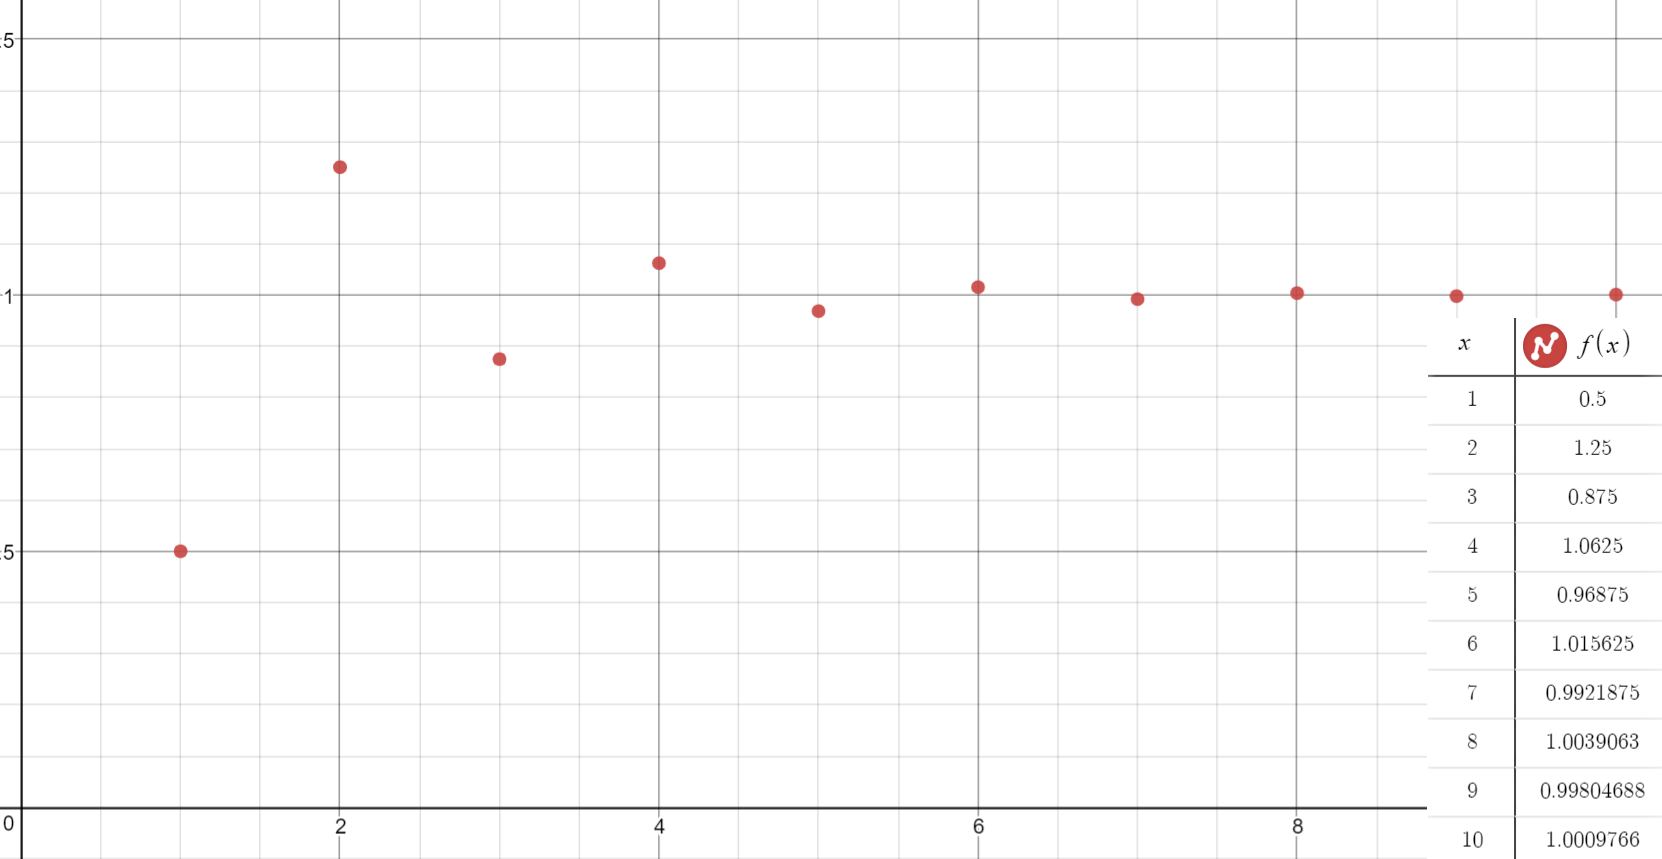
\includegraphics[width=\textwidth]{21}
    \end{align*}
        The sequence converges to 1.
    \begin{align*}
       \lim_{n\to\infty}\left(1+\left(-\frac{1}{2}^n\right)\right) = 1 + 0
    \end{align*}     
    \addtocounter{enumi}{3}\item $\frac{n^4}{n^3-2n}$
    \begin{align*}
        \lim_{n\to\infty}\frac{n^4}{n^3-2n}\cdot\frac{\frac{1}{n^3}}{\frac{1}{n^3}} = \lim_{n\to\infty}\frac{n}{1-\frac{1}{n^2}} = \frac{\infty}{1-0} = \infty \text{ Diverges}
    \end{align*}
    \newpage\addtocounter{enumi}{3}\item $a_n=e^{-1/\sqrt{n}}$
    \begin{align*}
        \lim_{n\to\infty} e^{-1/\sqrt{n}} = e^0 = 1 \text{ Converges}
    \end{align*}
    \addtocounter{enumi}{3}\item $a_n=\frac{n^2}{\sqrt{n^3+4n}}$
    \begin{equation*}
        \lim_{n\to\infty}a_n=\lim_{n\to\infty}\frac{n^2}{n^\frac{1}{2}\sqrt{n^2+4}} = \lim_{n\to\infty}\frac{n^\frac{3}{2}}{\sqrt{n^2+4}}=\lim_{n\to\infty}\frac{n^\frac{3}{2}}{\sqrt{n^2}}=\lim_{n\to\infty}n^\frac{1}{2}=\infty \text{ Diverges}
    \end{equation*}
    \addtocounter{enumi}{3}\item $\left\{\frac{(2n-1)!}{(2n+1)!}\right\}$\
    \begin{equation*}
        \lim_{n\to\infty}\frac{(2n-1)!}{(2n+1)(2n)(2n-1)!}=\lim_{n\to\infty}\frac{1}{(2n+1)(2n)} = 0 \text{ Converges}
    \end{equation*}
    \addtocounter{enumi}{3}\item $\{n^2e^{-n}\}$
        \begin{align*}
            \lim_{n\to\infty}a_n=\lim_{n\to\infty}\frac{n^2}{e^n}\stackrel{H}{=}\lim_{n\to\infty}\frac{2}{e^n}=0 \text{ Converges}
        \end{align*}
    \addtocounter{enumi}{3}\item $a_n=n\sin(1/n)$
    \begin{align*}
        a_n&=\lim_{n\to\infty}\frac{\sin{\frac{1}{n}}}{\frac{1}{n}} & x &= \frac{1}{n} ...\\
        &=\lim_{x\to 0}\frac{\sin{x}}{x}\stackrel{H}{=}0
        &\lim_{x\to 0}\frac{\cos{x}}{1}&=1 \text{ Converges}
    \end{align*}
    \addtocounter{enumi}{3}\item $a_n=\ln{(2n^2+1)}-\ln{(n^2+1)}$
    \begin{align*}
        \lim_{n\to\infty}\ln{\left(\frac{2n^2+1}{n^2+1}\right)}=\lim_{n\to\infty}\ln{\left(\frac{2+\frac{1}{n^2}}{1+\frac{1}{n^2}}\right)} = \ln{(2)} \text{ Converges}
    \end{align*}
    \addtocounter{enumi}{3}\item $\left\{0,1,0,0,1,0,0,0,1,...\right\}$\\\\
    The sequence infinitely alternates between 0 and 1 with infinitely increasing intervals. Therefore, it is impossible to find the limit, making it inherently divergent.\newpage
    Determine whether the sequence is increasing, decreasing, or not monotonic. Is the sequence bounded?
    \addtocounter{enumi}{19}\item $a_n=\frac{1}{2n+3}$\\\\
    The sequence is decreasing as n approaches $\infty$. The sequence is also bounded between 0 and $\frac{1}{5}$.
    \addtocounter{enumi}{1}\item $a_n=n(-1)^n$\\\\
    The sequence is increasing as n approaches $\infty$. The sequence is also not bounded since it alternates between signs and and approaches $\infty$ on both bounds.
    

\end{enumerate}

\newpage\section{11.1 II Sequences and Convergence}
\begin{enumerate}
    \item Consider the sequence $\left\{\frac{n}{n+1}\right\}_{n=1}^\infty$ which converges to the limit L =1.
    \begin{enumerate}
        \item Using the $\epsilon$ - definition of convergence of a sequence, prove that this sequence does in fact converge to this limit.
        \\\\ For any $\epsilon > 0$ there is an $N > 0$ such that $n > N$ then $|a_n-1| < \epsilon$\\
        \\Suppose that $\epsilon > 0$:
        \begin{align}
            |a_n-1| &< \epsilon\\
            \left|\frac{n}{n+1}-\frac{n+1}{n+1}\right| &< \epsilon\\
            \left|\frac{-1}{n+1}\right| &< \epsilon\\
            \frac{1}{n+1} &<\epsilon\\
            \frac{1}{\epsilon}-1 &<n
        \end{align}
        For $N = \frac{1}{\epsilon}-1$ the sequence converges. 
        \item Using your work in part a) above, for each part below find the smallest value of N for the given value of $\epsilon$.
        \begin{enumerate}
            \item $\epsilon=.25$
                \begin{equation*}
                    \frac{1}{.25}-1 = 3
                \end{equation*}
            \item $\epsilon=.1$
                \begin{equation*}
                    \frac{1}{.1}-1 = 9
                \end{equation*}
            \item $\epsilon=.001$
                \begin{equation*}
                    \frac{1}{.001}-1 = 999
                \end{equation*}
        \end{enumerate}
    \end{enumerate}
\end{enumerate}
    

\end{document}
